% Define the document class
\documentclass[automatic-bibliography]{univsciauth}

% Load some extra packages
\usepackage{multirow}
\usepackage{longtable}
\usepackage{siunitx}

% Define the references file
\addbibresource{references.bib}

% Document specific configs
\title{Extension of Dasgupta's Technique for Higher Degree Approximation}
\shorttitle{Dasgupta's Technique}

\author[1]{P. L. Powar}
\author[1]{Rishabh Tiwari}
\author[2]{Vishnu Narayan Mishra*}
\authormail{vishnunarayanmishra@gmail.com}
\shortauthor{Powar et al.}

\Affil{1}{Department of Mathematics and Computer Science, R.D. University, Jabalpur, 482001, (M.P.), India.}
\Affil{2}{Department of Mathematics, Indira Gandhi National Tribal University, Lalpur, Amarkantak, Anuppur, Madhya Pradesh 484 887, India.}

\funding{n.a.}
\esmaterial{Supp. 1}

\doi{10.11144/Javeriana.SC26-2.eodt}

% Start writing your document
\begin{document}
% \setcounter{page}{139}
\maketitle
\thispagestyle{firstpage}

\begin{abstract}
In the present paper, rational wedge functions for degree two approximation have
been computed over a pentagonal discretization of the domain, by using an
analytic approach which is an extension of Dasgupta\rq{}s approach for linear
approximation. This technique allows to avoid the computation of the exterior
intersection points of the elements, which was a key component of the technique
initiated by Wachspress. The necessary condition for the existence of the
denominator function was established by Wachspress whereas our assertion,
induced by the technique of Dasgupta, assures the sufficiency of the existence.
Considering the adjoint (denominator) functions for linear approximation
obtained by Dasgupta, invariance of the adjoint for degree two approximation is
established. In other words, the method proposed by Dasgupta for the
construction of Wachspress coordinates for linear approximation is extended to
obtain the coordinates for quadratic approximation. The assertions have been
supported by considering some illustrative examples.

\keywords{Adjoint; invariance; pentagonal discretization; wedge functions.}
\end{abstract}

\section{Introduction}
Augustus Ferdinand M\"obius~\cite{mo} is attributed for initializing the concept
of Barycentric coordinates. Initially, it was restricted to a triangle in two
dimensional space. Generalization of these coordinates was first introduced by
Wachspress~\cite{wach71} where the concept was extended from triangles to convex
polygons, polycons~\cite{wach73} and further to 3-D elements~\cite{warren, wach,
wachs}. Meanwhile, there have been efforts to present simpler and general form
of barycentric coordinates~\cite{1,2,3,4,5,6} which may be computed and applied
easily.

It has become a trend as well as a need to machine the calculation of geometric
shapes and bodies using computers. Expansion of computer capacity has increased
computational sophistication leading to methods with more precision and less
time consumption and having newer fields of applications such as generalized
barycentric coordinates on irregular polygons~\cite{7}, interpolants within
convex polygons~\cite{das}, integration within polygonal finite
elements~\cite{9}, interpolations for temperature distributions~\cite{10}, in
the field of computer graphics, computational mechanics~\cite{11}, etc. To
obtain the desired shape using computers, the usual process is to interpolate
the provided data using a certain class of functions. The Finite Element Method
(FEM) algorithm in interpolation adds more perfection, as it allows to design by
fragmenting the given function or data which is to be approximated with respect
to the elements of the domain and then considering each fragment independently.

Wachspress' coordinates (cf.~\cite{wach}) in addition, provides inter-element
continuity, thus emerges as boon to shape formation. In this method
(see~\cite{wachs}), the domain is discretized using convex polygons called
elements, corresponding to each element, a basis of rational wedge functions is
defined for linear approximation.

In the Wachspress\rq{} method, the computation of rational wedge functions
relied on the geometry of the element under consideration, especially the
denominator of the wedge functions (adjoint) was the curve passing through the
exterior intersection points (EIPs) of the polygonal element. Thus, for each
element of the domain, EIPs are to be calculated to obtain the adjoint,
increasing the number of steps of the computation.

Dasgupta~\cite{das} simplified the task by proposing an analytic method for the
calculation of the adjoint to the wedge functions. The rational wedge functions
introduced by Wachspress~\cite{wachs} for the discretization with convex
polygons of order $m$ in a degree $k$ approximation are of the form
\begin{equation}
  \frac{P^{m+k-3}(x,y)}{P^{m-3}(x,y)} \label{eqn111}
\end{equation}
where $P^n(x,y)$ denotes a bivariate polynomial of degree  $n$. It has been
identified in~\cite{das} that the adjoint is nothing but the sum of numerators
of the wedge functions, having coefficients of terms of higher degree (higher
than $m-3$, cf. \autoref{eqn111}) equated to zero.

Dasgupta~\cite{das}, considered the rational wedge functions for degree one
approximation over a pentagonal discretization of the domain. In this paper, a
formulation to compute wedge functions for degree two approximation has been
proposed. It has been concluded that the adjoint function so computed is
invariant, i.e., adjoints of quadratic wedge functions are the same as those of
linear wedge functions. Also, they have been compared with the Wachspress\rq{}
wedge functions and observed to be the same.

It may be noted that wedge functions for degree two approximation provide better
approximant than the wedge functions for degree one approximation as the number
of nodal points is increased and so is the precision.

In this paper, the work of Dasgupta~\cite{das} has been extended as follows:
\begin{itemize}
  \item Dasgupta has imposed a constraint on the element that no side of
        the element should pass through the origin, whereas this paper covers the
        general case.
  \item The existence and uniqueness problem of the adjoint function has
        been studied in this paper which yields certain geometric conditions on the
        element for the existence of a unique adjoint function.
\end{itemize}

An algorithm based on a Mathematica program has been included in this paper,
which identifies the geometric constraints of a particular element and also
computes the approximation to the provided data. It is quite significant to note
that the denominator involved in the wedge construction due to Wachspress was
the curve passing through the exterior intersection points (EIP) of the convex
polygon of the mesh, whereas Dasgupta's approach computes the denominator
(adjoint) analytically without using the geometry of the element and later
assures that the adjoint essentially passes through the EIP, thus establishing
sufficiency of the condition for the existence of the denominator function,
making it a well-defined one.

\section{Prerequisites}\label{sec2}
In this section, some preliminaries which are needed for construction and
analysis are recalled.

Consider a closed and convex polygon $P_m = (1,2,\ldots,m)$, $m \geq 4$, with
$m$ vertices as nodes in $\mathbb{R}^2$. Let $i-1$ and $i$ be the consecutive
nodes of $P_m$ and $i \in \mathbb{Z}_m$, where $\mathbb{Z}_m$ is the set of
integers modulo $m$.

\begin{definition}
  \emph{Discretization}~\cite{phi} of the domain
  $\Omega \subseteq \mathbb{R}^2$ using convex polygons is the process of
  subdividing $\Omega$ into non overlapping polygons $P_m$ in such a way that:
        \begin{itemize}
          \item The union of all polygons in the discretization is equal
                to the domain $\Omega$.
          \item The intersection of interiors of any two elements is an empty
                set.
          \item The boundaries of any two elements intersect only at a
                common edge or at a common node.
          \item The domain is simply connected.
        \end{itemize}
\end{definition}

\begin{definition}[\cite{wachs}, see also~\cite{wach}]
  Sides of the polygon containing the node $i$, are called \emph{adjacent}
  to $i$ and remaining sides are called \emph{opposite} to the node $i$.
\end{definition}

\begin{definition}[\cite{wachs}, see also~\cite{wach}]
  Let $s_{i}$ be the straight line passing through the nodes $i-1$ and $i$
  where Cartesian coordinates of $i-1$ and $i$ are $(x_{i-1},y_{i-1})$ and
  $(x_i,y_i)$ respectively. Then, the \emph{linear form} of the line $s_i$ is
  denoted by
  \begin{equation}\label{r1}
    l_i\cong l_i(x,y)=(i-1,i)\cong (x-x_i)(y_{i-1}-y_i)-(y-y_i)(x_{i-1}-x_i).
  \end{equation}
\end{definition}

\begin{definition}[\cite{wachs}, see also~\cite{wach}]
  The \emph{wedge function} corresponding to the $i$\textsuperscript{th} node of
  $P_m$ is a regular function $N_i: P_m \rightarrow \mathbb{R}$ of the form
  \begin{eqnarray}
    N_i(x,y)= K_i\frac{P^{m+k-3}(x,y)}{P^{m-3}(x,y)},\quad (i\in\mathbb{Z}_m)\label{eq1}
  \end{eqnarray}
  where $P^n(x,y)$ is a bivariate polynomial of degree $n$.
\end{definition}

We now enumerate the properties of wedge functions described in~\cite{wachs}.

\textbf{Properties of wedge functions for degree one approximation}\:\cite{wachs}
In order to obtain a linear approximation corresponding to an element, the class
of wedge functions described in~\cite{wachs} satisfies the following properties:
\begin{enumerate}
  \item There is a node at each vertex of the polygon. For each node there is an
        associated wedge within each polygon containing the node.
  \item Wedge $N_i(x,y)$ associated with node $i$ is normalized to unity at $i$
        ($i\in\mathbb{Z}_m$).
  \item Wedge $N_i(x,y)$ is linear on sides adjacent to $i$
        ($i\in\mathbb{Z}_m$).
  \item{\label{4_2}} Wedge $N_i(x,y)$ vanishes on sides opposite to node
        $i$.
  \item{\label{5_2}} The wedges associated with $P_m$ form a basis for
        degree one approximation over it. For the polygon $P_m$, there must be at least
        $m$ nodes. For these to suffice, we must have (cf.~G.15 of~\cite{das1}):
        \begin{align}
          &\sum_{i=1}^{m}N_i(x,y) = 1, \label{2.1_1}\\
          &\sum_{i=1}^{m}x_iN_i(x,y) = x,\\
          &\sum_{i=1}^{m}y_iN_i(x,y) = y.
        \end{align}
  \item Each wedge function and all its derivatives are continuous within the polygon
        for which the wedge is a basis function.
\end{enumerate}

\begin{definition}[\cite{wachs}]
  If the domain under consideration is discretized using pentagons then each
  pentagon of the domain is termed as a \emph{pentagonal element} (or simply an
  element).
\end{definition}

\begin{definition}[\cite{wachs}]
  The node on a side of the polygon, such that it does not coincide with
  the vertices is said to be a \emph{side node}.
\end{definition}

\section{Construction of wedge functions}\label{sec3}
Referring to \autoref{eq1}, the wedge functions for degree one and two
approximation over a pentagonal element are  computed in this section.

\subsection{Degree one approximation}

\subsubsection{Construction}

Applying the technique of Dasgupta (cf.\,\cite{das}) and referring the
generalized form of wedge functions (cf. \autoref{eq1}), we now determine the
adjoint to the linear approximation over $P_5$.

The wedge functions $N_i^1$\rq{}s corresponding to the nodes of $P_5$
(cf.~\autoref{p4}) have been defined as follows:
\begin{equation}
  \begin{aligned}\label{d2}
    N_1^1&=K_1\frac{l_{3}l_{4}l_{5}}{D(x,y)},
    &N_2^1&=K_2\frac{l_{1}l_{4}l_{5}}{D(x,y)},
    &N_3^1=K_3\frac{l_{1}l_{2}l_{5}}{D(x,y)},\\
    N_4^1&=K_4\frac{l_{3}l_{2}l_{1}}{D(x,y)},
    &N_5^1&=K_5\frac{l_{3}l_{4}l_{2}}{D(x,y)}.
  \end{aligned}
\end{equation}
Where $K_i$'s are appropriate normalizing constants.
\begin{figure}[t!]
  \centering
  \scalebox{0.70}{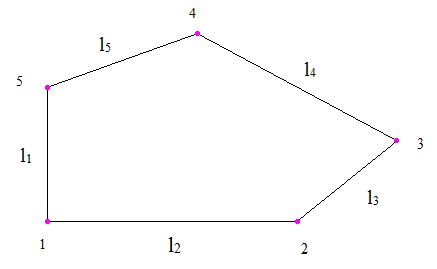
\includegraphics{figures/p4.jpg}}
  \caption{Pentagon}\label{p4}
\end{figure}

In view of~\cite{das} and value of $\{N_i^1\}_{i=1}^5$ the denominator $D(x,y)$
can be obtained by following steps 1, 2, and 3:
\paragraph{\textbf{Step 1}} Normalize $K_1$ to 1 (cf. \autoref{d2}).
\paragraph{\textbf{Step 2}} Sum the numerators of all the $N_i^1$'s.
\paragraph{\textbf{Step 3}} In the above sum, equate the coefficients of terms
of higher degree (higher than two) to zero and obtain a system of linear
equations
\begin{equation}
  \mathbf{AK=M},\label{deg1sys}
\end{equation}
where $\mathbf{A}$ is a $4\times4$ coefficient matrix,
$\mathbf{K=\left[\begin{array}{cccc}K_2&K_3&K_4&K_5\end{array}\right]^T}$ and
\textbf{M} is a $4\times1$ matrix of some real numbers.
On solving this system of linear equations the denominator has been obtained (cf.\,\cite{das}).
\subsubsection{Existence}

Our aim in this section is to obtain a solution of the system of linear
equations (\autoref{deg1sys}). A unique solution to the system will exist if the
determinant of $\mathbf{A}$ is non-zero. Consider $\Omega$ to be the pentagonal
discretization of the domain $\mathbb{R}^2$ (cf.~\autoref{fig1}).

The following theorem establishes the conditions under which a unique solution
to the system (\autoref{deg1sys}) exists.

\begin{figure}[b!]
  \centering
  \scalebox{0.50}{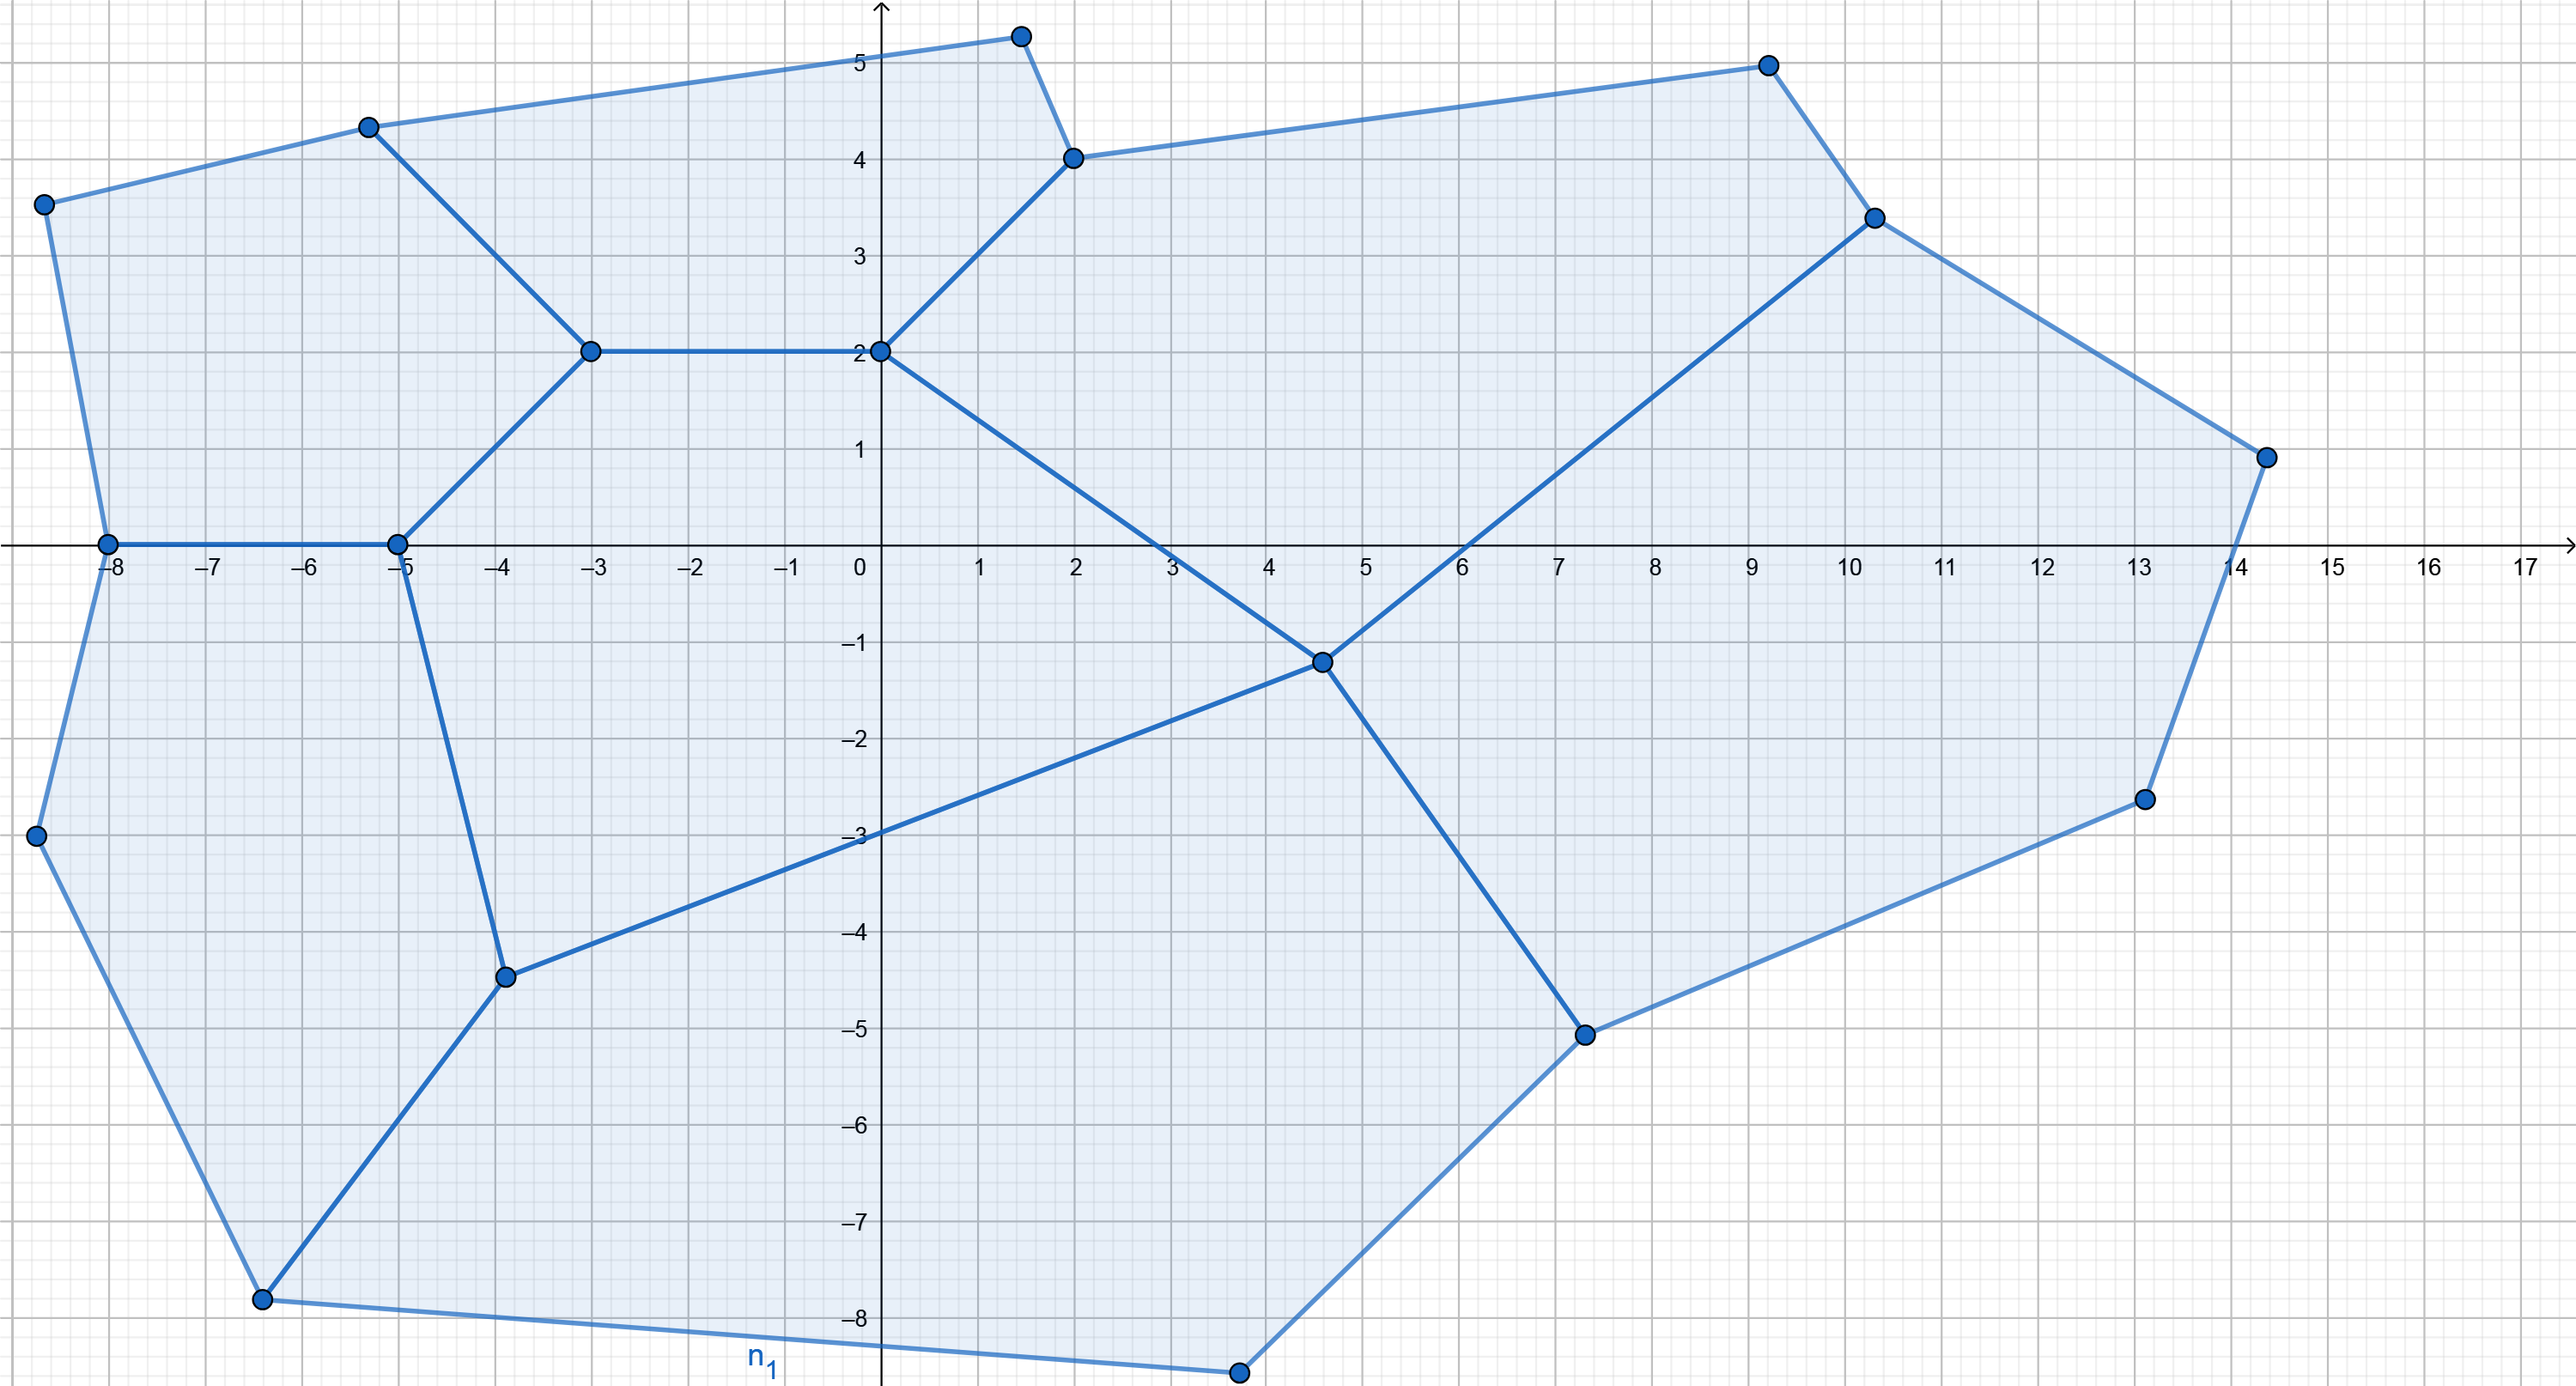
\includegraphics{figures/pent_disc1.png}}
  \caption{Pentagonal discretization}\label{fig1}
\end{figure}

\begin{theorem}
  Let $\Omega \subseteq \mathbb{R}^2 $ be the pentagonal discretization of the
  domain and $P_5^1$ is an arbitrary element of $\Omega$. Then the adjoint of the
  wedge  functions for degree one approximation corresponding to the element
  $P_5^1$ exists and is unique if the following conditions hold:
  \begin{itemize}
    \item[{\upshape(A)}] No two sides of $P_5^1$ are parallel.
    \item[{\upshape(B)}] No three vertices of $P_5^1$ are co-linear.
  \end{itemize}
\end{theorem}
\begin{proof}
  Consider the pentagon $P_5^1= (a,b,c,d,e)$ having Cartesian coordinates of the
  vertices as $(a_1,a_2)$, $(b_1,b_2)$, $(c_1,c_2)$, $(d_1,d_2)$, and $(e_1,e_2)$
  respectively. Without any loss of generality, the pentagon $P_5^1$ can be
  transformed into the pentagon $P_5=(1,2,3,4,5)$, having Cartesian coordinates
  $(0,0)$, $(x_2,0)$, $(x_3,y_3)$, $(x_4,y_4)$, and $(x_5,y_5)$ (cf.~\autoref{fig2}).
  \begin{figure}[b!]
    \centering
    \scalebox{0.60}{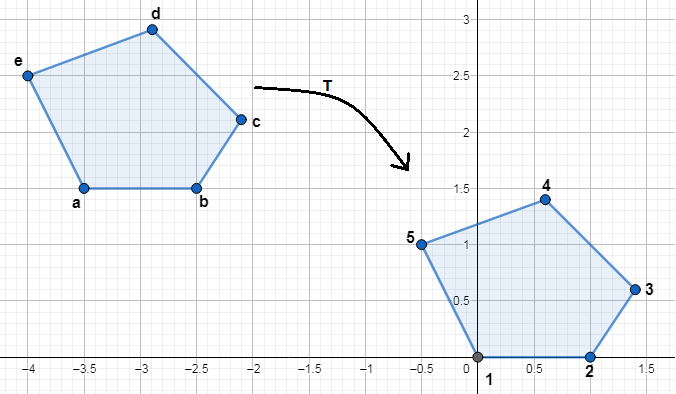
\includegraphics{figures/pent_transformation11.png}}
    \caption{Transformation of the element}\label{fig2}
  \end{figure}

  Using the notation of linear forms described in Section~2, we now consider the
  following:
  \begin{equation}
    \begin{aligned}
      l_1&=(5,1)\cong x_5 y - x y_5, \\
      l_2&=(1,2)\cong y, \\
      l_3&=(2,3)\cong -(-x_2 + x_3) y + x y_3 - x_2 y_3 \\
      l_4&=(3,4)\cong -(x_3 + x_4) y + x_4 y_3 - x (y_3 - y_4) - x_3 y_4, \\
      l_5&=(4,5)\cong-(-x_4 + x_5) y+ x_5 y_4 - x (y_4 - y_5) - x_4 y_5.
    \end{aligned}
  \end{equation}
  In view of wedge properties, the numerator of the wedge function corresponding
  to the $i$\textsuperscript{th} node $\text{Num}_i$, for (say) $i=1,\ldots,5$,
  will be:
  \begin{equation}
    \begin{aligned}
      \mathrm{Num}_1&=K_1l_3l_4l_5, & \mathrm{Num}_2&=K_2l_4l_1l_5, & \mathrm{Num}_3=K_3l_1l_2l_5,\\
      \mathrm{Num}_4&=K_4l_1l_2l_3, & \mathrm{Num}_5&=K_5l_2l_3l_4.
    \end{aligned}
  \end{equation}
  Using relation \autoref{eq1}, and applying the technique prescribed
  in~\cite{das} we  equate the coefficients of terms $x^i y^j$ ($i+j=3$,
  $i,j=0,1,2,3$) to zero. Thus, normalizing the constant $K_1 $ to 1, a system
  having four equations in four unknowns viz $\{ K_i \}_{i=2}^5$, of the form
  $\mathbf{AK=M}$ (cf. \autoref{deg1sys}) is obtained. It may be verified easily
  that a unique solution to this system will exist only if the following
  conditions hold:
  \begin{itemize}
    \item $x_3 \neq x_2$,
    \item $y_3\neq y_4$,
    \item $ x_4 \neq \dfrac{-x_2y_4+x_3y_4+x_2y_5-x_3y_5}{y_3}$,
    \item $x_3\neq x_4$.
  \end{itemize}
  The above conditions in turn imply assertions (A) and (B).
\end{proof}

\subsection{Degree two approximation}

In order to define the wedge functions for degree two approximation the
following construction will be required:
\subsubsection{Construction}

\begin{figure}[b!]
  \centering
  {\tikz\node[inner sep=0pt,label={[anchor=north west]north west:\subref{fig:4a}}] {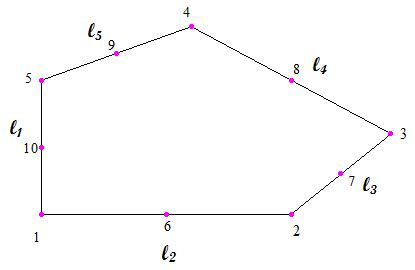
\includegraphics[scale=0.58]{figures/p6.jpg}}; \phantomsubcaption\label{fig:4a}}
  \qquad
  {\tikz\node[inner sep=0pt,label={[anchor=north west]north west:\subref{fig:4b}}] {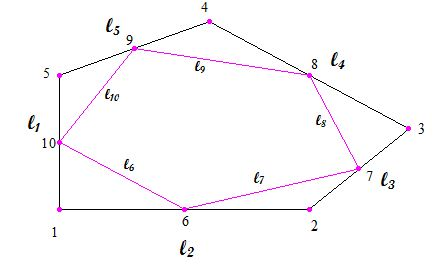
\includegraphics[scale=0.58]{figures/p7.jpg}}; \phantomsubcaption\label{fig:4b}}
  \caption{\subref{fig:4a} Side Nodes. \subref{fig:4b} Linear forms of straight lines through side nodes}\label{p7}
\end{figure}

Define side nodes $i+5$ ($i=1,2,\ldots,5$) on the line joining nodes $(i,i+1)$,
$i\in\mathbb{Z}_5$. The linear form of the straight line joining nodes $i$ and
$i+1$ (by convention node11 $=$ node6) is denoted by $l_{i+1}$,
$i = 6, 7, 8, 9$, and $10$ (cf.~\autoref{fig:4b}) which satisfies the equation
$l_{i+1}=0$ on this line.

Inheriting the process of computation of wedge functions for linear
approximation (see~\cite{das1}), the following wedge properties for degree two
approximation over $P_m$ have been considered.

{\textbf{Properties of wedge functions for degree two approximation.}}
In order to obtain a quadratic approximation corresponding to an element $P_m$,
the class of wedge functions satisfy the following properties:
\begin{enumerate}
  \item{} There is a node at each vertex of the polygon and the side nodes
        on the sides of the polygon. For each node (vertex node and side node) there is
        an associated wedge within each polygon containing the node.
  \item{} Wedge $N_i(x,y)$ associated with node $i$ is normalized to unity
        at node $i$.
  \item{} Wedge $N_i(x,y)$ is quadratic on sides adjacent to $i$.
  \item{\label{4_1}} Wedge $N_i(x,y)$ vanishes on sides opposite to node
        $i$ and at all nodes $j$ for which $j\neq i$.
  \item{\label{5_1}} The wedges associated with $P_m$ form a basis for
        approximation of degree two over it. There must be at least $m$ nodes and $m$
        side nodes in the polygon $P_m$. For these to suffice, we must have:
        \begin{equation}
          \begin{aligned}\label{2.1}
            &\sum_{i=1}^{2m}N_i(x,y) =1, &&\sum_{i=1}^{2m}x_iN_i(x,y) =x,\\
            &\sum_{i=1}^{2m}y_iN_i(x,y) =y, &&\sum_{i=1}^{2m}x_i^2N_i(x,y) =x^2,\\
            &\sum_{i=1}^{2m}y_i^2N_i(x,y) =y^2, &&\sum_{i=1}^{2m}x_iy_iN_i(x,y) =xy,
          \end{aligned}
        \end{equation}
        where $(x_i,y_i)$ is a Cartesian coordinate of the vertex $i$ of
        $P_m$.
  \item{} Each wedge function and all its derivatives are continuous
        within the polygon for which the wedge is a basis function.
\end{enumerate}

In view of the aforesaid properties the wedge function corresponding to the
$i$\textsuperscript{th} node ($i\in\mathbb{Z}$) of $P_5$ will be,
\begin{equation}\label{eqn21}
        N^2_i (x,y) = \begin{cases} \dfrac{K_iL_il_{5+i}}{Q(x,y)}, & \hbox{for } i \leq 5,\\
    \vspace{0pt}\\
    \dfrac{K_iL_{i-5}l_{i-5}}{Q(x,y)}, & \hbox{for } 5 < i \leq 10,\end{cases}
\end{equation}
where
\begin{equation}
  L_i  = \prod_{\mathclap{j = 1, j \neq i, j \neq i+1}}^{5} l_j \label{eqn1'}\qquad\mbox{(by convention }l_6=l_1).
\end{equation}

\subsubsection{Computation of adjoint}

Following the technique of Dasgupta~\cite{das}, the unknowns
$\{ K_i \}_{i=2}^{10}$ are to be computed, to determine the adjoint function
$Q(x,y)$ for degree two approximation.

In view of \autoref{eqn21} and \autoref{eq1}, it is evident that to achieve
degree two approximation, $Q(x,y)$ must be a bivariate polynomial of degree two.

Hence in view of the above assertion, the technique of Dasgupta (cf.~\cite{das})
has been applied in the following steps:

\paragraph{\textbf{Step 1}} By property \ref{5_2},
\begin{equation}
  \sum_{i=1}^{10}N_i^2(x,y) =1, \label{eqn10}
\end{equation}
where $N_i^2(x,y)$ is defined in \autoref{eqn21}.

\paragraph{\textbf{Step 2}} With reference to \autoref{eqn10}, the sum of
numerators of the rational forms $N_i^2(x,y)$ is held on the left and is equated
with $Q(x,y)$.

\paragraph{\textbf{Step 3}} In relation \autoref{eq1}, it is quite clear that
the coefficients of terms of degree higher than 2 must be equated to zero and,
without loss of generality, the constant $K_1(\neq0) $ may be normalized to 1.

Thus, nine linear equations (with nine unknowns $\{ K_i \}_{i=2}^{10}$) are
left, which can be expressed in matrix form as
\begin{equation}
  \mathbf{AK=M},\label{7}
\end{equation}
where $\mathbf{A}$ is a $9\times9$ square matrix,
$\mathbf{K=\left[\begin{array}{ccccccccc}K_2&K_3&K_4&K_5&K_6&K_7&K_8&K_9&K_{10}\end{array}\right]^T}$
and $\mathbf{M}$ is a $9\times1$ matrix of some real numbers.

The aim is to compute the adjoint $Q(x,y)$, for which using \autoref{7} the
values of $K_i$'s are needed to be computed.

On solving these equations, if the solution exists, the values of $K_i$'s are
obtained and thus the exact value of $Q(x,y)$.

\section{Invariance of Adjoint}\label{sec4}
In this section, the adjoints obtained by applying the technique of Dasgupta
(cf.\,\cite{das}) in Section~3, are compared with the denominator function
introduced by Wachspress (see~\cite{wachs}).

The concept of computing adjoints by using the `exterior intersection point'
(EIP) was initiated by Wachspress~\cite{wach}, where an EIP is the point of
intersection of the extended opposite sides of the pentagon which do not
intersect within it (cf.~\autoref{p8}).
\begin{figure}[b!]
  \centering
  \scalebox{0.70}{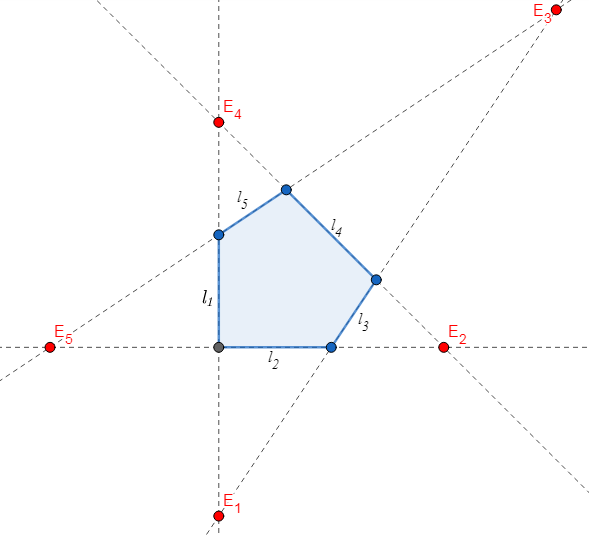
\includegraphics{figures/p91.png}}
  \caption{Pentagon representing exterior intersection points}\label{p8}
\end{figure}
In \autoref{p8}, $E_1$, $E_2$, $E_3$, $E_4$, and $E_5$ are the EIPs.

According to Wachspress~\cite{wach} the denominator function for the wedge
construction of degree one over a pentagon, is a unique curve of degree two,
passing through the five EIPs.

It was observed that the adjoint computed by the method of Dasgupta for Linear
approximation and by Wachspress' EIP method are identical. In fact, even on
increasing the degree of approximation the adjoint remains unchanged.

\begin{theorem}
  For a pentagonal discretization $\Omega$ of the domain, the adjoint function
  computed by Wachspress' method is the same as that obtained by Dasgupta for
  degree one approximation. Moreover, the adjoint remains unchanged for degree two
  approximation, computed by inheriting the technique of Dasgupta.
\end{theorem}
\begin{proof}
  According to Wachspress, the adjoint for linear approximation over a
  pentagon is a unique curve represented by a degree two polynomial which passes
  through the EIPs.

  Let $D^*(x,y)$ be the denominator function of the wedge obtained by
  Wachspress method, $D(x,y)$ be the adjoint function obtained by Dasgupta's
  technique for degree one approximation, and $Q(x,y)$ the adjoint function
  obtained for degree two approximation by the technique of Dasgupta.

  It can be seen easily that the EIP $E_i$, is the intersection of the
  lines $l_i = 0$ and $l_{i+2} = 0$, $i=1, \ldots,5$ (here $l_6=l_1$ and
  $l_7=l_2$). Consider,
  \begin{equation}
    D(x,y) = \sum_{i=1}^{5} \mathrm{Num}^1_i(x,y) =  \sum_{i=1}^5 K_il_{i+2}l_{i+3}l_{i+4} \
    \mbox{(cf.~Section~3)}\label{c1}
  \end{equation}
  and,
  \begin{equation}
    Q(x,y) = \sum_{i=1}^{10} \mathrm{Num}^2_i(x,y) =  \sum_{i=1}^5 K_iL_il_{n+i} + \sum_{i=6}^{10}  K_iL_{i-5}l_{i-5} \ \mbox{ (cf.~Section~4)}\label{2}
  \end{equation}
  and either $l_i$ or $l_{i+2}$ is present in each component of the sum in the
  right side of \autoref{c1} and \autoref{2}.

  Hence,
  \begin{equation}
    D(x,y)|_{E_i}=Q(x,y)|_{E_i}=0\quad (i=1,\ldots,5).
  \end{equation}
  It implies that
  \begin{equation}
    D(x,y)\cong Q(x,y)\cong D^*(x,y).
  \end{equation}
\end{proof}

\section{Numerical Examples}\label{sec5}
In order to support the assertions, made in this paper an illustrative example
is discussed here. The example is organized as follows:
\begin{enumerate}
  \item{\label{1}} Linear approximation over the given pentagon is computed for
        the function $\sin(xy)$.
  \item Considering the same function $\sin(xy)$, degree two approximation
        has been computed on the pentagon as described in \autoref{1}.
\end{enumerate}

\begin{example}
  Consider the pentagon $P_5 =(1,2,3,4,5)$ with Cartesian coordinates of
  the vertices as (cf. \autoref{fig3}) $1=(0,0)$, $2=(1,0)$,
  $3=\left(\frac{7}{5},\frac{3}{5}\right)$,
  $4=\left(\frac{3}{5},\frac{7}{5}\right)$ and $5=(0,1)$.
\end{example}

\paragraph{\textbf{Degree one approximation}} In reference to \autoref{deg1sys},
it is noticed that $|A|\neq 0$, hence the adjoint $D(x,y)$ exists uniquely, and
\begin{equation}
  D(x,y)=\frac{1}{125}\left(24 x^2 - 32 x y+24 y^2-12 x-12 y-72\right).\label{e2}
\end{equation}
\begin{figure}[t!]
  \centering
  \scalebox{1.4}{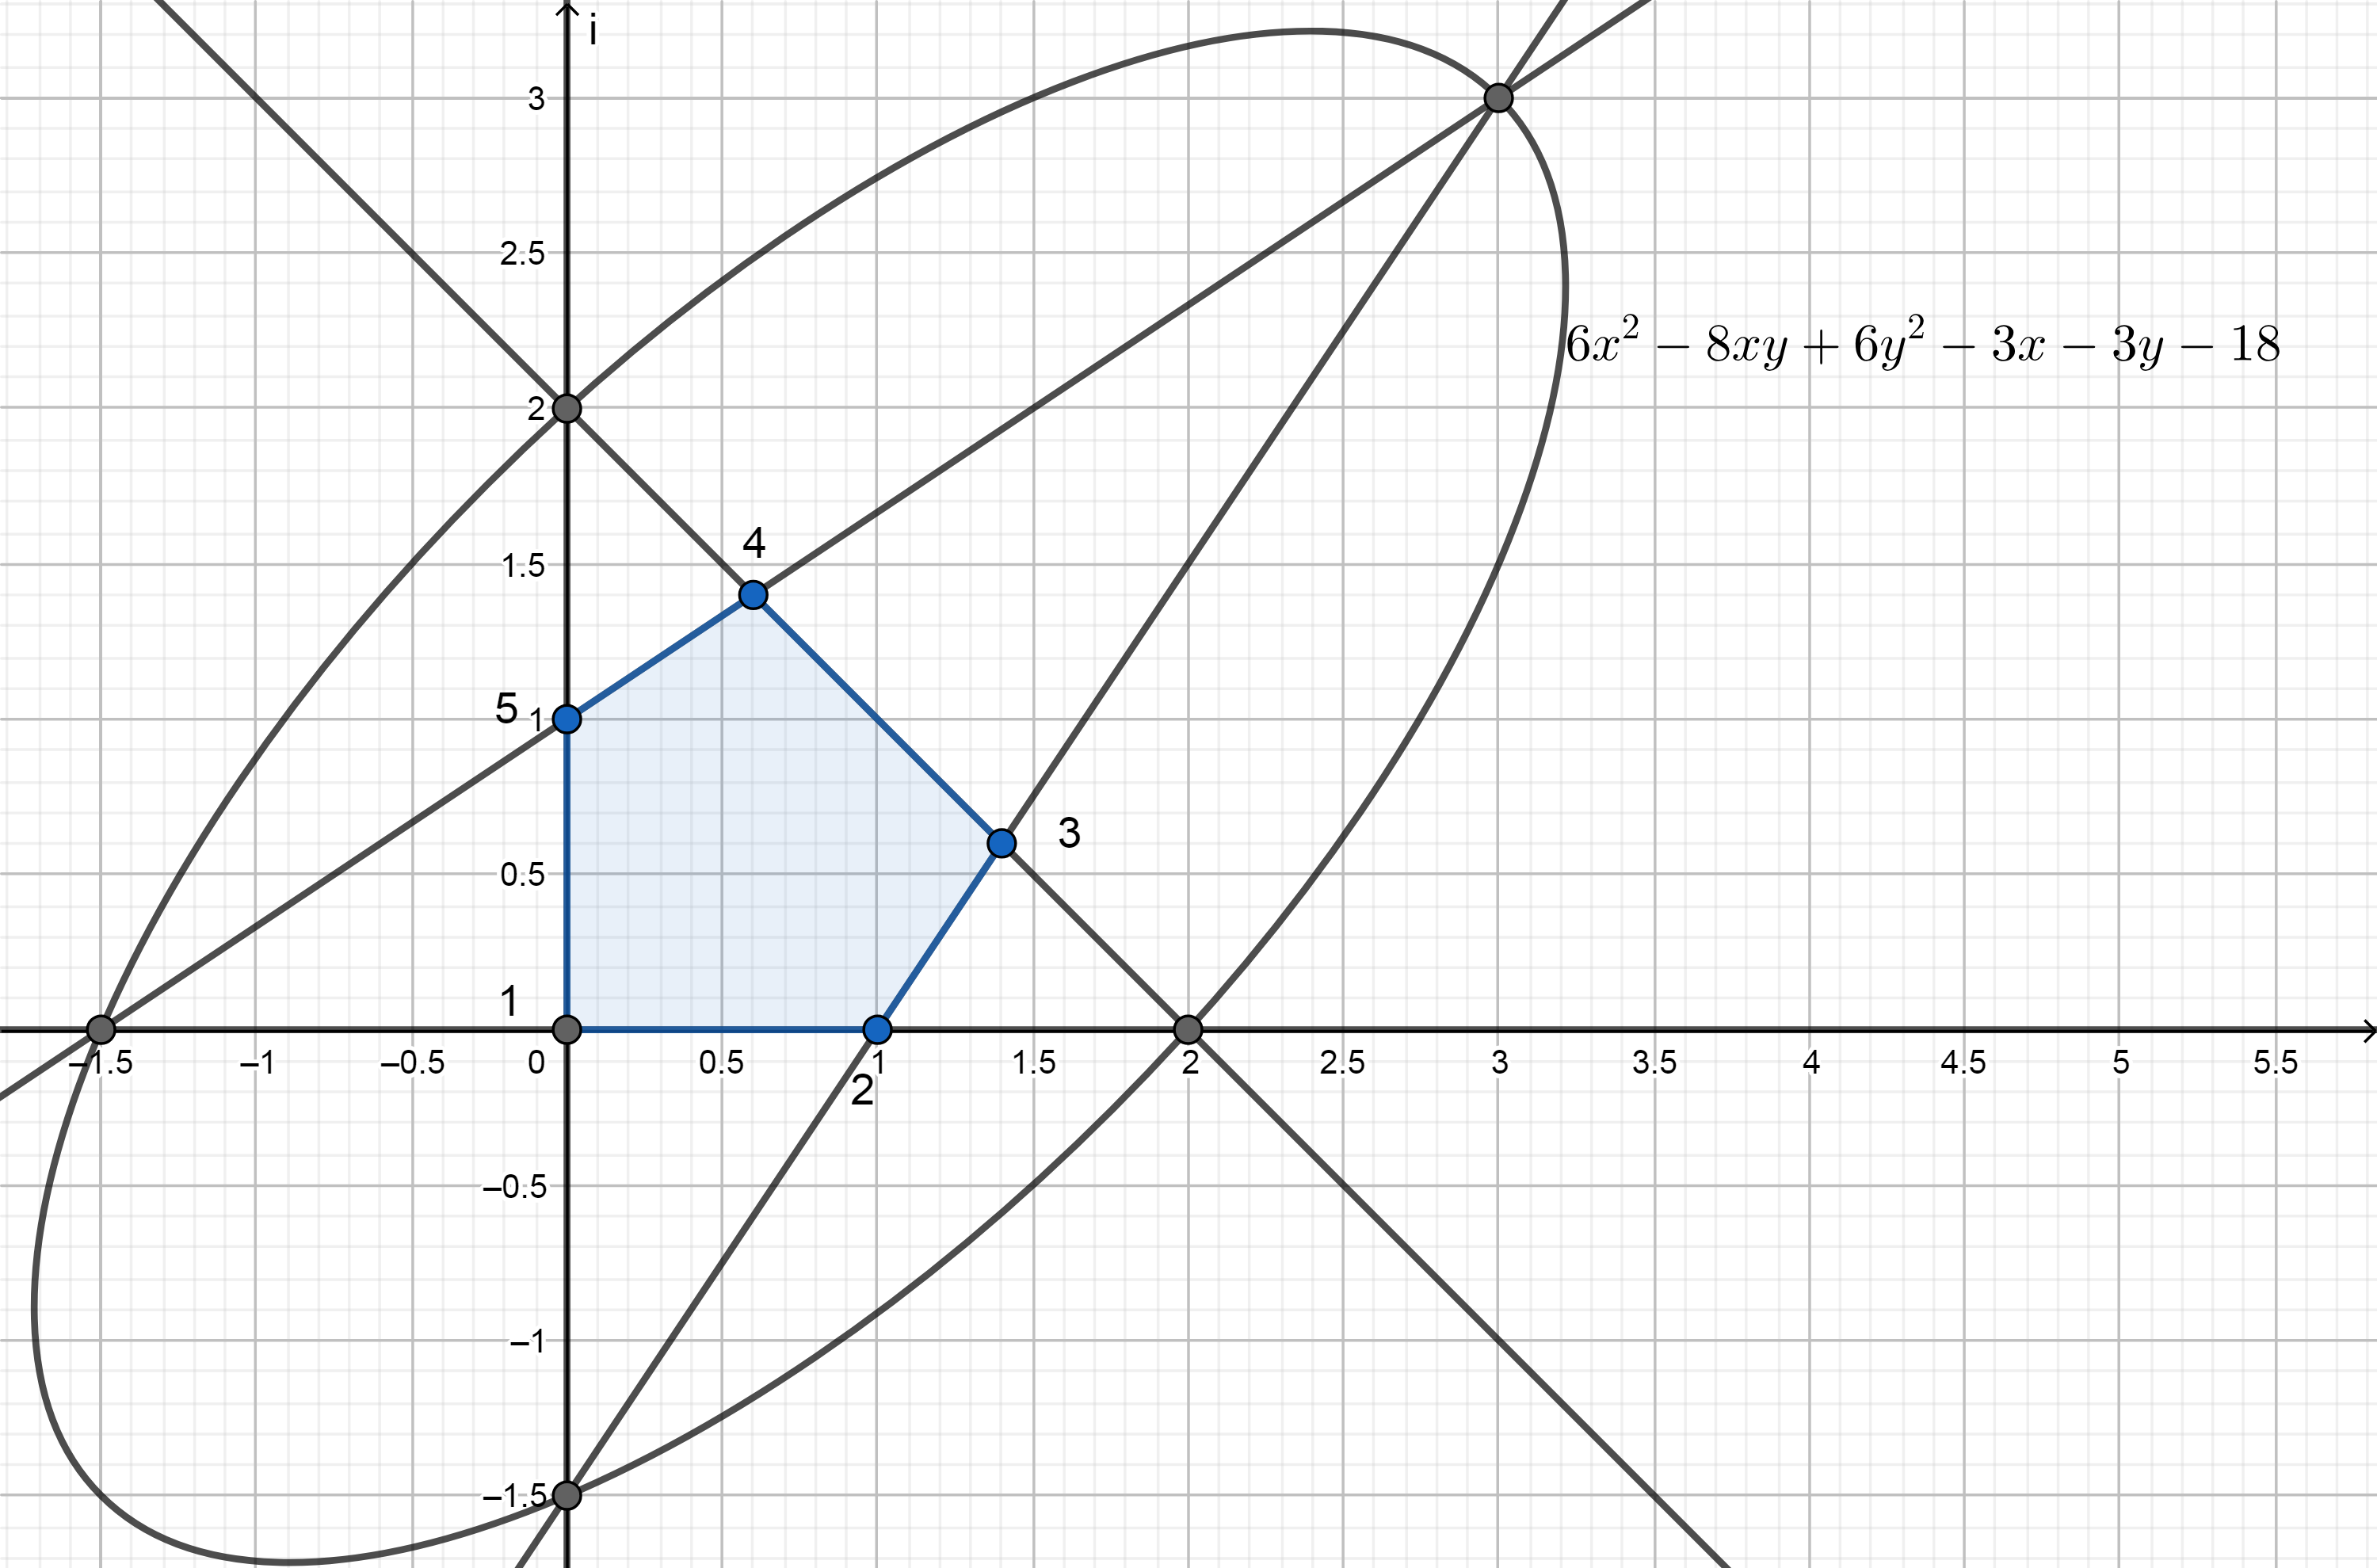
\includegraphics{figures/pent_EIP_curve.png}}
  \caption{Pentagon with EIPs and curve}\label{fig3}
\end{figure}

For a non linear function, say $f(x,y)=\sin(xy)$, the approximant is
\begin{equation}
  \phi(x,y)=\frac{5xy (-6 + x + y) \sin(21/25)}{6x^2 - 8xy + 6y^2 - 3x - 3y -18}.
\end{equation}
The function $f(x,y)$ over the element $P_5$ and its approximation is displayed
in \autoref{fig5}.
\begin{figure}[H]
  \centering
  {\phantomsubcaption\label{fig:7a}}
  {\phantomsubcaption\label{fig:7b}}
  \tikz\node[inner sep=8pt,label={[anchor=north west]north west:\subref{fig:7a}}] {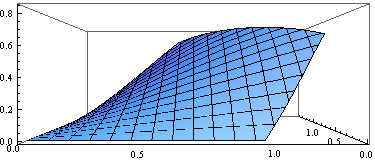
\includegraphics[scale=0.58]{figures/sin(xy).png}};
  \qquad
  \tikz\node[inner sep=6pt,label={[anchor=north west]north west:\subref{fig:7b}}] {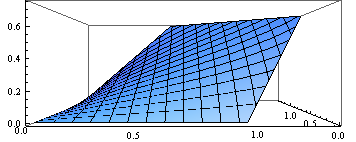
\includegraphics[scale=0.65]{figures/deg1.png}};
  \caption{Comparison of the original curve and its linear approximation. \subref{fig:7a} Function $\sin(xy)$. \subref{fig:7b} Degree one approximation of $\sin(xy)$}\label{fig5}
\end{figure}

\paragraph{\textbf{Degree two approximation}}
In order to define wedge functions for degree two approximations, the
intermediate points with the following Cartesian coordinates on sides of the
pentagon $P_5$ are introduced:
$6=\left(\frac{1}{2},0\right)$, $7=\left(\frac{12}{10},\frac{3}{10}\right)$,
$8=(1,1)$, $9=\left(\frac{3}{10},\frac{12}{10}\right)$ and
$10=\left(0,\frac{1}{2}\right)$ (cf.~\autoref{fig7}).

In view of~\autoref{7}, the adjoint exists uniquely, and is given by
\begin{equation}
  Q(x,y)=\frac{1}{125}(6 x^2 - 8 x y+6 y^2-3 x-3 y-9).\label{e1}
\end{equation}
\begin{figure}[t!]\centering
        \scalebox{1.1}{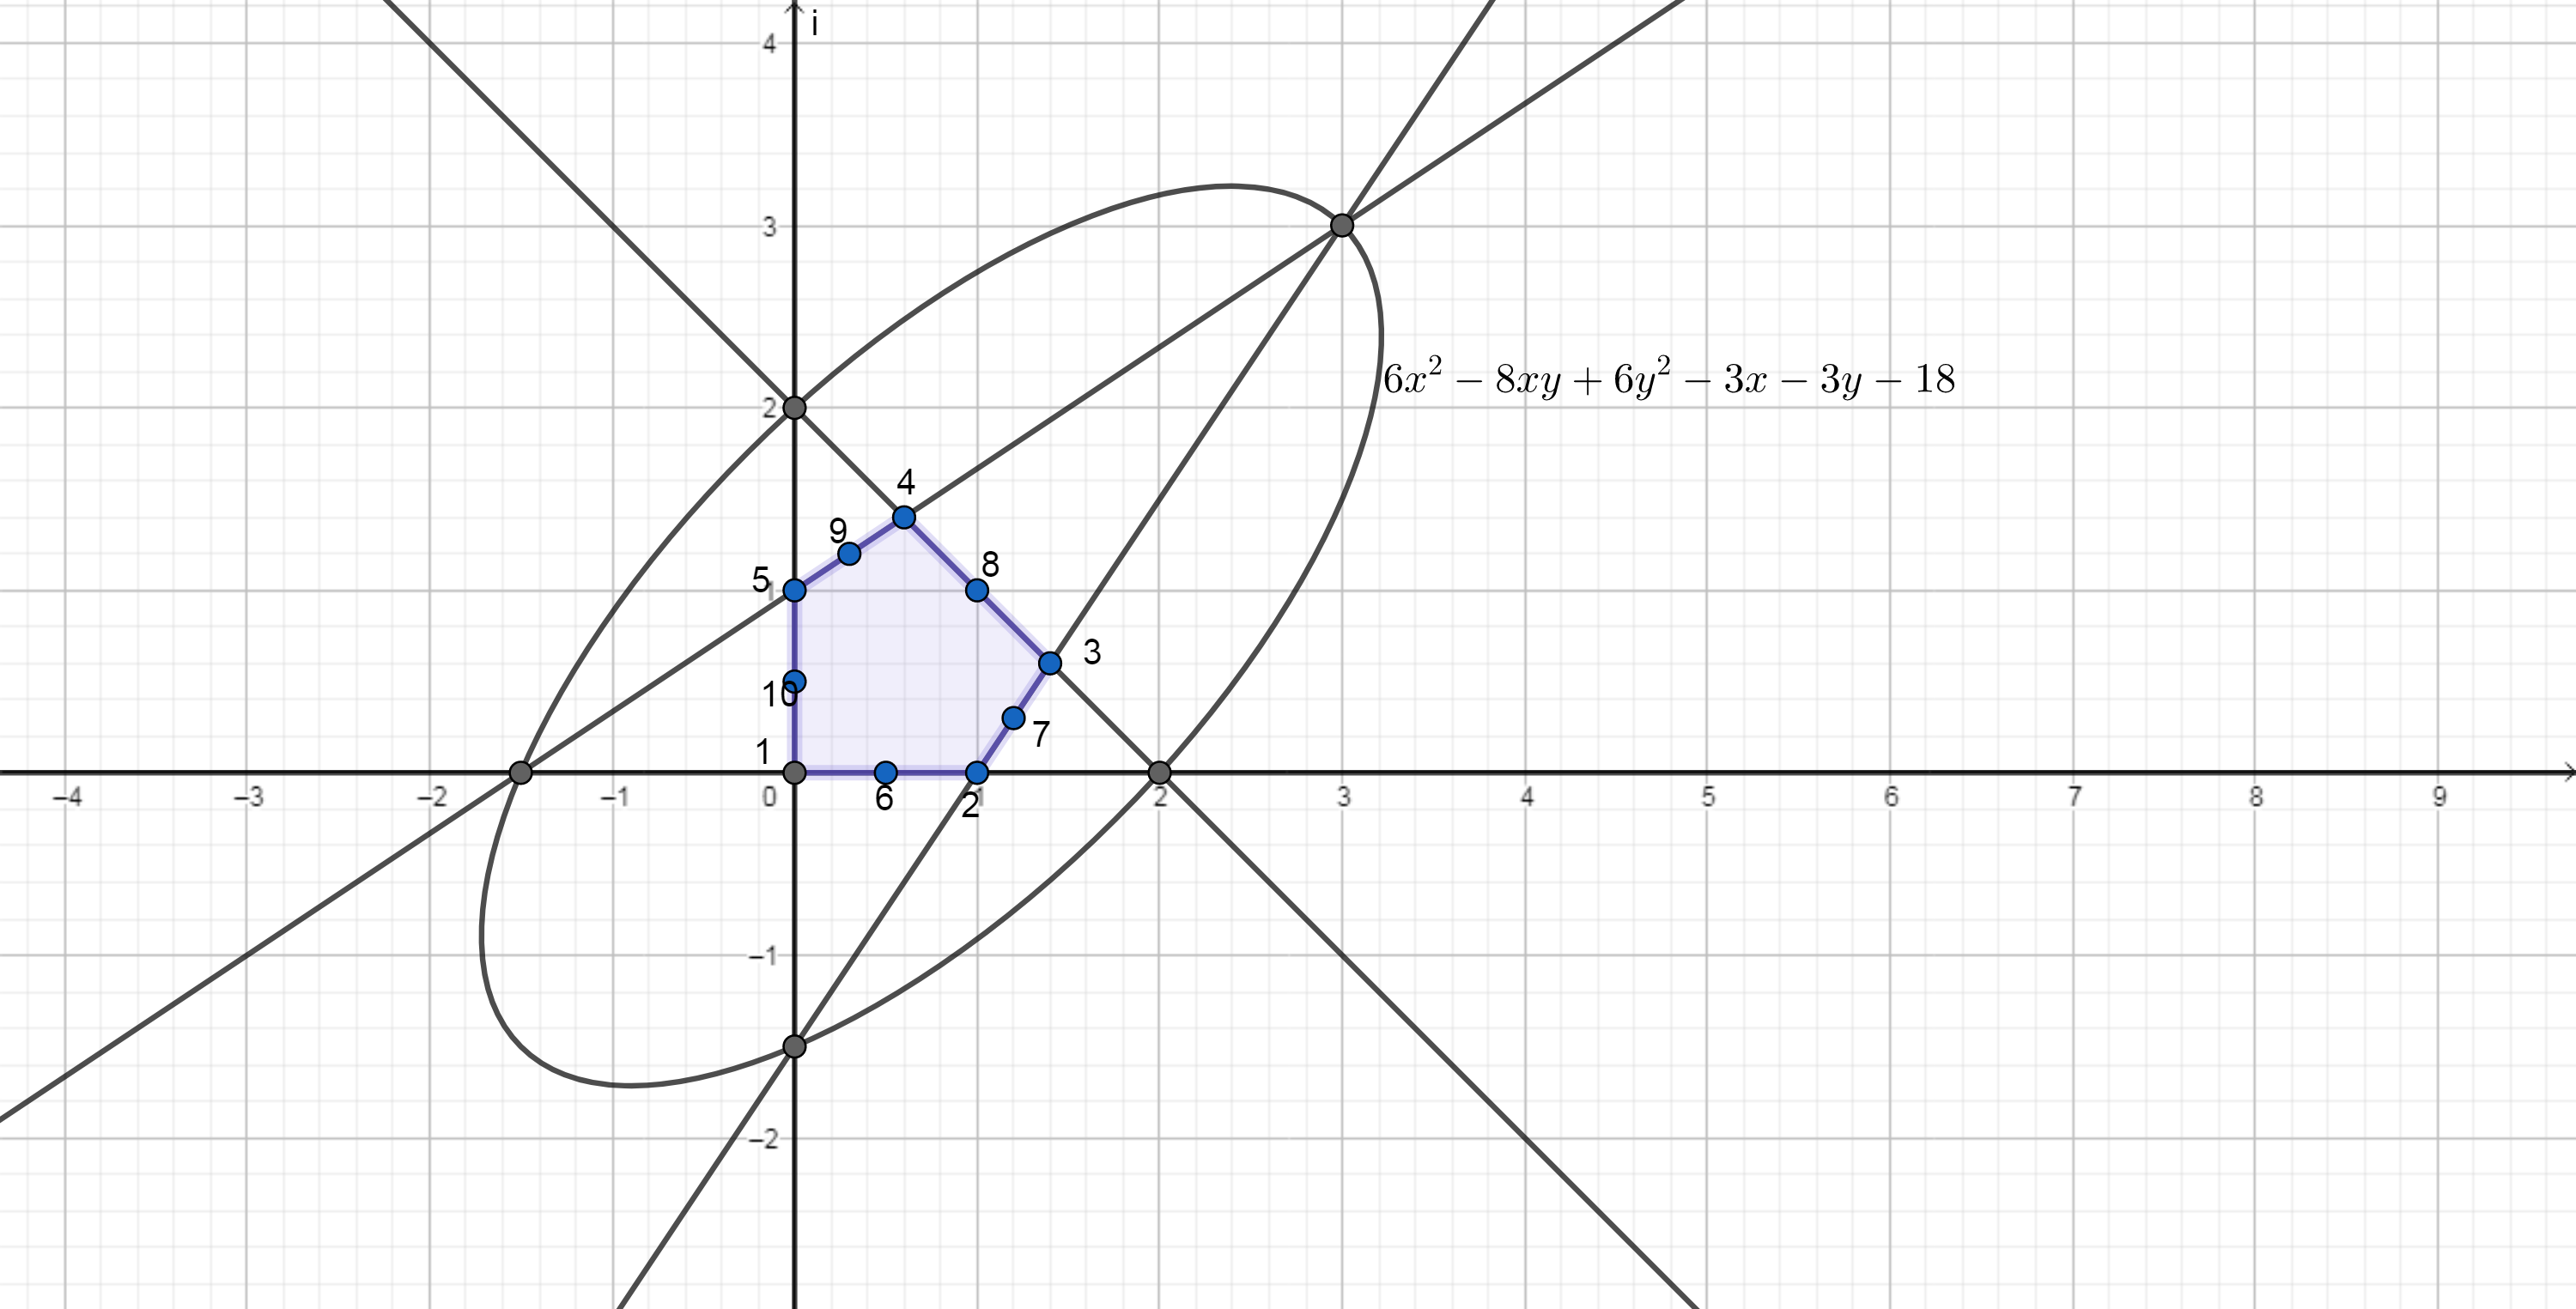
\includegraphics[trim={0 0 3cm 0},clip]{figures/pent_int_curve1.png}}
  \caption{Pentagon with intermediate points, EIPs and curve}\label{fig7}
\end{figure}

For the same function $f(x,y)=\sin(xy)$ the approximant, say $\psi(xy)$, is
obtained as
\begin{multline}
  \psi(x,y) = \frac{5xy}{6x^2 -8xy +6y^2 - 3x -3y -18}\biggl[{-4(-6 +x +y)(-2 +x +y)\sin\left(\frac{9}{25}\right)} \\
  \hspace{2cm} - {(-27 + 4x^2 + x(18 - 17y) + 2y (9 + 2y)) \sin\left(\frac{21}{25}\right)} \\
  + {(3 + 2x - 3y) (-3 + 3x - 2y) \sin(1)}\biggr].
\end{multline}
The function $f(x,y)$ over the element $P_5$ and its approximation is displayed
in \autoref{fig51}.
\begin{figure}[t!]
  \centering
  {\phantomsubcaption\label{fig:9a}}
  {\phantomsubcaption\label{fig:9b}}
  \tikz\node[inner sep=10pt,label={[anchor=north west]north west:\subref{fig:9a}}] {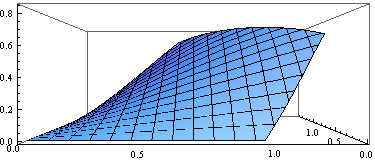
\includegraphics[scale=0.60]{figures/sin(xy).png}};
  \qquad
  \tikz\node[inner sep=10pt,label={[anchor=north west]north west:\subref{fig:9b}}] {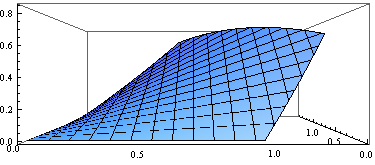
\includegraphics[scale=0.60]{figures/deg2.png}};
  \caption{Comparison of the original curve its degree two approximation. \subref{fig:9a} Function $\sin(xy)$. \subref{fig:9b} Degree two approximation of $\sin(xy)$}\label{fig51}
\end{figure}
From \autoref{e2} and \autoref{e1} it can be seen that the adjoint is invariant.

\subsection{Comparative Study}
In order to compare the linear and the quadratic approximations over the
considered element we have computed the error, which is defined as follows:
\begin{equation}
  \|e\| =\int_{\omega}|f(x,y)-A(x,y)|\,dxdy, \quad \text{where $A$ is the approximate value of $f$.}
\end{equation}
\begin{itemize}
        \item Error for linear approximation $= \num{0.0366299}$.
        \item Error for quadratic approximation $= \num{0.012876}$.
\end{itemize}

It is clear from the above computation that the quadratic approximation is
closer to the function in comparison to the linear approximation.

\begin{remark}
  Comparing \autoref{fig5} and \autoref{fig51}, it may be observed that the
  degree two approximation is quite close to the given function $f(x,y)=\sin(xy)$.
\end{remark}

\section{Algorithm to compute the degree two approximation\label{sec6}}
An algorithm based on a program written in Mathematica is placed in this part of
the paper, which illustrates the method for computing the approximant.

\subsection{Description of the algorithm}

\noindent{\\\textbf{Step 2}\:} In this step we declare the variables, to assign
the coordinates of the polygon as well as the edge nodes.

\noindent{\textbf{Step 3}\:} Computes the linear forms, of all the edges.

\noindent{\textbf{Step 4}\:} Multiply the linear forms and get a polynomial of
degree four in the numerator, namely, $\text{num}[(xy),[i]]$, $i=1,2,\ldots,10$,
corresponding to each node.

\noindent{\textbf{Step 5}\:} Define denominator as the sum of all the numerators
num[$(xy),[i]$].

\noindent{\textbf{Step 6}\:} In the denominator polynomial, equate the
coefficients of the terms of degree higher than two to zero.

\noindent{\textbf{Step 7}\:} Solve the system of $9\times9$ equations obtained
in Step 6, to get $k_i$'s.

\noindent{\textbf{Step 8}\:} Finally get the denominator polynomial and the
wedge functions.

\noindent{\textbf{Step 9}\:} Compute the error in approximation, i.e., integrate
the modulus of difference in approximate and approximant over the considered
element.

\section{Conclusion}
The method developed by Dasgupta gives a new approach to solving problems
related to rational FEM. Being a technique different from the well established
Wachspress\rq{} method, it gives a new perspective to the rational finite
element methods with a scope of rebuilding the theory with the emergence of some
new concepts, applications, and mainly easy computation of the denominator
function. The theorem stated in this paper identifies the constraints in the
geometry of the element required to be taken care of, to assure the existence of
the wedge functions.

In addition to the conditions for the existence of the wedge functions, a method
to compute wedge functions for degree two approximation has been proposed, a
theorem has been stated claiming invariance of the adjoint functions in moving
from degree one to degree two approximation; also the adjoint function is
compared with the adjoint of Wachspress wedge functions and found to be the
same. Wedge functions for degree two approximation increase the precision in
approximation.

\section{Conflict of Interest}
The authors certify that they have no affiliations with or involvement in any
organization or entity with any financial interest (such as honoraria;
educational grants; participation in speakers membership, employment,
consultancies, stock ownership, or other equity interest; and expert testimony
or patent arrangements), or non (such as personal or professional relationships,
affiliations, knowledge or beliefs) in the subject matter or materials discussed
in this manuscript. The authors declare that there are no conflicts of interest.

\printbibliography

\clearpage

\begin{shaded*}
  {\fontsize{11}{10}\selectfont\textbf{\textcolor{myseccolor}{Extensión de la Técnica de Dasgupta para Aproximación de Grado Superior}}}

  \vspace{3mm}

  {\fontsize{11}{10}\selectfont\textbf{\textcolor{myseccolor}{Resumen:}}}
  En el presente artículo, se calculan funciones racionales para aproximación de grado dos sobre una
  discretización pentagonal del dominio, utilizando un enfoque analítico que es una extensión del enfoque
  de Dasgupta para la aproximación lineal. Esta técnica permite evitar el cálculo de los puntos de
  intersección exteriores de los elementos, que es un componente clave de la técnica iniciada por
  Wachspress. La condición necesaria para la existencia de la función del denominador fue establecida por
  Wachspress mientras que nuestra afirmación, inducida por la técnica de Dasgupta, asegura la suficiencia
  de la existencia. Considerando las funciones adjuntas (denominador) para aproximación lineal obtenidas
  por Dasgupta, se establece la invariancia del adjunto para la aproximación de grado dos. En otras
  palabras, el método propuesto por Dasgupta para la construcción de coordenadas de Wachspress para
  aproximación lineal se amplía para obtener las coordenadas para aproximación cuadrática. Las
  afirmaciones se sustentan considerando algunos ejemplos ilustrativos.

  {\fontsize{11}{10}\selectfont\textbf{\textcolor{myseccolor}{Palabras Clave:}}}
  Adjunto; invarianza; discretización pentagonal; funciones tipo cuña.
\end{shaded*}

\begin{shaded*}
  {\fontsize{11}{10}\selectfont\textbf{\textcolor{myseccolor}{Extensão da Técnica de Dasgupta para Aproximação de Grau Superior}}}

  \vspace{3mm}

  {\fontsize{11}{10}\selectfont\textbf{\textcolor{myseccolor}{Resumo:}}}
  No presente artigo, funções racionais para aproximação de grau dois são calculadas sobre uma
  discretização pentagonal do domínio, usando uma abordagem analítica que é uma extensão da
  abordagem de Dasgupta para aproximação linear. Esta técnica permite evitar o cálculo dos pontos de
  intersecção exteriores dos elementos, componente chave da técnica iniciada pelo Wachspress. A
  condição necessária para a existência da função denominadora foi estabelecida por Wachspress
  enquanto nossa assertiva, induzida pela técnica de Dasgupta, assegura a suficiência da existência.
  Considerando as funções adjuntas (denominador) para aproximação linear obtidas por Dasgupta, a
  invariância da adjunta para aproximação de grau dois é estabelecida. Em outras palavras, o método
  proposto por Dasgupta para a construção de coordenadas Wachspress para aproximação linear é
  estendido para obter as coordenadas para aproximação quadrática. As afirmações são apoiadas
  considerando alguns exemplos ilustrativos.

  {\fontsize{11}{10}\selectfont\textbf{\textcolor{myseccolor}{Palavras-chave:}}}
  Adjunto; invariância; discretização pentagonal; funções de cunha.
\end{shaded*}
\clearpage

\begin{shaded*}
  {\fontsize{11}{10}\selectfont\textbf{\textcolor{myseccolor}{P. L. Powar}}}

  Professor P. L. Powar (Retd.) received her M.Sc. and Ph.D. in Mathematics form Rani Durgavati
  University, Jabalpur, India. Her research areas are Cutting Stock Problem, Spline Approximation Theory,
  Finite Element Methods, Fixed Point Theory, Topology and Software Engineering.

  ORCID: \href{https://orcid.org/0000-0002-6332-9386}{0000-0002-6332-9386}
\end{shaded*}

\vspace{5mm}
\begin{shaded*}
  {\fontsize{11}{10}\selectfont\textbf{\textcolor{myseccolor}{Rishabh Tiwari}}}

  Rishabh Tiwari is currently working in the Department of Mathematics, Rani Durgavati University,
  Jabalpur, India. He has received M. Sc., M. Phil and Ph. D. in Mathematics from Rani Durgavati University,
  Jabalpur, India. His research areas are, Algebraic Topology, Finite Element Methods and Topology.

  ORCID: \href{https://orcid.org/0000-0001-7097-9777}{0000-0001-7097-9777}
\end{shaded*}

\vspace{5mm}
\begin{shaded*}
  {\fontsize{11}{10}\selectfont\textbf{\textcolor{myseccolor}{Vishnu Narayan Mishra}}}

  Dr. Vishnu Narayan Mishra is working as Professor and Head of Department of Mathematics at Indira
  Gandhi National Tribal University, Lalpur, Amarkantak, Madhya Pradesh, India. Prior to this, he also held as
  academic positions as Assoc. Prof. at IGNTU, Amarkanta, Assistant Professor in AMHD, SVNIT, Surat. He
  received the Ph.D. degree in Mathematics from Indian Institute of Technology, Roorkee in 2007. His
  research interests are in the areas of pure and applied mathematics including Approximation Theory,
  Nonlinear analysis and Optimization etc.

  ORCID: \href{https://orcid.org/0000-0002-2159-7710}{0000-0002-2159-7710}
\end{shaded*}

\end{document}
